\documentclass[aps,apl,twocolumn,groupedaddress]{revtex4-1}
%\documentclass[12pt]{article}   	% use "amsart" instead of "article" for AMSLaTeX format

\usepackage{graphicx}				% Use pdf, png, jpg, or eps� with pdflatex; use eps in DVI mode
								% TeX will automatically convert eps --> pdf in pdflatex		
\usepackage{caption}

\begin{document}

\title{Classical Schr\"{o}dinger-like Equation Revisited}
\author{Chris Richardson, Peter Schlagheck, John Martin, Thierry Bastin}
\affiliation{University of Liege}
\date{\today}							% Activate to display a given date or no date

\begin{abstract}

A wave equation which sheds light on the origin of the Schr\"{o}dinger equation has previously been proposed.  This equation which we call the classical Schr\"{o}dinger-like equation is the Schr\"{o}dinger equation plus an extra non-linear term, a classicality-enforcing potential, which has the effect of canceling out all quantum and wave-like effects.  The Schr\"{o}dinger equation has been recovered from the classical Schr\"{o}dinger-like equation by making assumptions which have the effect of completely canceling the classicality-enforcing potential.

We demonstrate both analytically and numerically that it is not strictly necessary to get rid of the classicality-enforcing potential to recover quantum behavior.  We show that by scaling and not necessarily eliminating the classicality-enforcing potential the linear Schr\"{o}dinger equation is recovered, but with a rescaled $\hbar$.  Even though the classical Schr\"{o}dinger-like equation with a scaled classicality-enforcing potential is non-linear, we demonstrate that it behaves in a very linear way.

We call the classical Schr\"{o}dinger-like equation with a scaled classicality-enforcing potential the transition equation and it can be a tool to explore the transition between the quantum and classical worlds.  We show that the results of an experiment involving quantum behavior at a macroscopic level can benefit from the use of the transition equation.

\end{abstract}

\maketitle

\section{Explaining the Classical Schr\"{o}dinger-like Equation}

The evolution of a classical particle can be described by its action $S(x,t)$ which obeys the the Hamilton-Jocobi equation:

\begin{eqnarray}
\frac{\partial S(x,t)}{\partial t} &=& \frac{1}{2 m} \nabla S(x,t)^2 - V \label{eqn:hamilton-jacobi}
\end{eqnarray}

If we assume instead that the particle has some statistical distribution in space given by $\rho(x,t) = A^2(x,t)$ we can construct a complex valued classical wave function:

\begin{eqnarray}
\psi_{cl}(x,t) &=& A(x,t) e^{\frac{i}{\hbar} S(x,t)} \label{eqn:classical_wf}
\end{eqnarray}

This wave function should obbey the continuity equation:

\begin{eqnarray}
\frac{\partial \rho}{\partial t} &=& - \nabla \cdot j \label{eqn:classical_wf} \nonumber \\
&=& - \nabla \cdot \frac{\hbar}{i m} \left(\psi^*_{cl} \frac{\partial \psi_{cl}}{\partial x} -  \frac{\partial \psi^*_{cl}}{\partial x} \psi_{cl} \right)
\end{eqnarray}

Which gives an equation derived separately by Schleich et al. which they refer to as the Van Vleck continuity equation.  

\begin{eqnarray}
\frac{\partial A^2(x,t)}{\partial t} + \frac{\partial}{\partial x} \left( \frac{1}{m} \frac{\partial S(x,t)}{\partial x} A^2(x,t) \right)= 0  \label{eqn:Oriols_cons}
\end{eqnarray}

Combining Eqs. (\ref{eqn:hamilton-jacobi}), (\ref{eqn:classical_wf}) and (\ref{eqn:Oriols_cons}) we get the classical Schr\"{o}dinger-like equation:

\begin{eqnarray}
i \hbar \frac{\partial \psi_{cl}}{\partial t} &=& - \frac{\hbar^2}{2 m} \frac{\partial^2 \psi_{cl}}{\partial x^2} \nonumber \\
&&+ \left(V + \frac{\hbar^2}{2 m} \frac{1}{\left| \psi_{cl} \right|} \frac{\partial^2 \left| \psi_{cl} \right|}{\partial x^2}\right) \psi_{cl} \label{eqn:class_schrod}
\end{eqnarray}

\section{A Classical Schr\"{o}dinger-like Equation}

A differential equation that describes classical (non-quantum, non-wave-like) physics has been derived by Bohm \cite{bib:bohm} and Oriols and Mompart \cite{bib:obm}.  Separately, Schleich et al. \cite{bib:revisited} have also derived the same equation and suggest that the Schr\"{o}dinger equation has its origins in it.  We call it the classical Schr\"{o}dinger-like equation and it is defined as:

\begin{eqnarray}
i \hbar \frac{\partial \psi_{cl}}{\partial t} &=& - \frac{\hbar^2}{2 m} \frac{\partial^2 \psi_{cl}}{\partial x^2} \nonumber \\
&&+ \left(V + \frac{\hbar^2}{2 m} \frac{1}{\left| \psi_{cl} \right|} \frac{\partial^2 \left| \psi_{cl} \right|}{\partial x^2}\right) \psi_{cl} \label{eqn:class_schrod}
\end{eqnarray}

Where the probability in analogy to the Schr\"{o}dinger equation is given from the modulus squared of $\psi$, the classical wave function.  Eq. (\ref{eqn:class_schrod}) is the Schr\"{o}dinger equation plus an extra non-linear term which has the effect of canceling out all quantum or wave-like effects.  Schleich et al. refer to this term as the \emph{classicality-enforcing potential}.  It is obvious that if this term were absent, Eq. (\ref{eqn:class_schrod}) reduces to the fully quantum Schr\"{o}dinger equation.

Schleich et al. transfer from this non-linear classical Schr\"{o}dinger-like equation to the linear Schr\"{o}dinger equation by associating the classicality-enforcing potential with the quantum action.  In this way, the classicality-enforcing potential is canceled out in Eq. (\ref{eqn:class_schrod}).

We would like to add, however, that it is not strictly necessary to get rid of the classicality-enforcing potential to recover quantum behavior.  We have found that by scaling and not necessarily eliminating the classicality-enforcing potential the linear Schr\"{o}dinger equation is recovered, but with a rescaled $\hbar$.

Inserting a degree of quantumness, $0 \leq \epsilon \leq 1$, into Eq. (\ref{eqn:class_schrod}) allows us to explore the smooth transition from the classical world, $\epsilon = 0$, to the quantum one, $\epsilon = 1$.

\begin{eqnarray}
i \hbar \frac{\partial \psi}{\partial t} &=& - \frac{\hbar^2}{2 m} \frac{\partial^2 \psi}{\partial x^2} + \left(V + (1 - \epsilon) \frac{\hbar^2}{2 m} \frac{1}{\left| \psi \right|} \frac{\partial^2 \left| \psi \right|}{\partial x^2}\right) \psi \label{eqn:class_schrod_ep}
\end{eqnarray}

We call this the transition equation and we will show that for all values of $\epsilon \neq 0$ it exhibits quantum behavior.  To demonstrate this we take three approaches.  First we show analytically that the transition equation is equivalent to the Schr\"{o}dinger equation with a rescaled $\hbar$.  We then we explore numerically what the effect of scaling the classicality-enforcing potential has on the double slit experiment.  Finally we explore how the transition equation can shed light on the results of a macroscopic quantum experiment.

\section{Scaling $\hbar$}

The non-linear transition equation is equivalent to the linear Schr\"{o}dinger equation with a $\hbar$ scaled by the degree of quantumness, $\epsilon$.

\begin{eqnarray}
\tilde{\hbar} = \hbar \sqrt{\epsilon} \label{eqn:hbar_scaled}
\end{eqnarray}

We show this by first writing the wave function in its polar form:

\begin{eqnarray}
\psi &=& A e^{\frac{i}{\hbar} S} \label{eqn:polarwf}
\end{eqnarray}

Where A and the action S are both real.  We then plug Eq. (\ref{eqn:polarwf}) into the transition equation, Eq. (\ref{eqn:class_schrod_ep}), and find the individual elements.  The Laplacian is:

\begin{eqnarray}
\nabla^2 \psi &=& (\nabla^2 A + 2 \frac{i}{\hbar}  (\nabla A) \cdot (\nabla S) \nonumber \\
&& + \frac{i}{\hbar} A \nabla^2 S - \frac{1}{\hbar^2}  A (\nabla S)^2) e^{\frac{i}{\hbar} S} 
\end{eqnarray}

The time derivative of Eq. (\ref{eqn:polarwf}) is:

\begin{eqnarray}
i \hbar \frac{\partial \psi}{\partial t} &=& (i \hbar \frac{\partial A}{\partial t} - A \frac{\partial S}{\partial t}) e^{\frac{i}{\hbar} S} 
\end{eqnarray}

And the contribution from the classicality-enforcing potential is:

\begin{eqnarray}
(1 - \epsilon) \frac{\psi}{\left| \psi \right|} \nabla^2 \psi &=& (1 - \epsilon) (\nabla^2 A) e^{\frac{i}{\hbar} S} 
\end{eqnarray}

Gathering the real and imaginary terms we recover the continuity equation:

\begin{eqnarray}
m \frac{\partial A}{\partial t}  &=& - (\nabla A) \cdot (\nabla S) - \frac{1}{2} A \nabla^2 S  \label{eqn:continuity}
\end{eqnarray}

and an equation very similar to the Hamilton-Jacobi equation but with a term scaled by the degree of quantumness, $\epsilon$:

\begin{eqnarray}
 \frac{\partial S}{\partial t} &=& \frac{1}{2 m} (\nabla S)^2 - V   +  \epsilon \frac{\hbar^2}{2 m} \frac{ \nabla^2 A}{A}
\end{eqnarray}

Making the substitution $\tilde{\hbar} = \hbar \sqrt{\epsilon}$ we get:

\begin{eqnarray}
\frac{\partial S}{\partial t} &=& \frac{1}{2 m} (\nabla S)^2 - V   +  \frac{\tilde{\hbar}^2}{2 m} \frac{ \nabla^2 A}{A}  \label{eqn:hamilton-jacobi_rescaled}
\end{eqnarray}

Which cancels out the degree of quantumness.  Eqs. (\ref{eqn:continuity}) and (\ref{eqn:hamilton-jacobi_rescaled}) are now completely equivalent to the Schr\"{o}dinger equation with a rescaled $\hbar$ and we can write:

\begin{eqnarray}
\psi &=& A e^{\frac{i}{\tilde{\hbar}} S} \\
i \tilde{\hbar} \frac{\partial \psi}{\partial t}  &=& -  \frac{\tilde{\hbar}^2}{2 m} \nabla^2 \psi + V \psi
\end{eqnarray}

It is possible to scale $\hbar$ directly in the Schr\"{o}dinger equation to explore the transition to the classical domain, but it becomes problematic as $\hbar \rightarrow 0$.  We can instead scale the degree of quantmness, $\epsilon$ in the transition equation to explore the transition to the classical world.  This does leave us with a non-linear equation to solve, but it avoids the problems that arise when using the Schr\"{o}dinger equation with a small $\hbar$.
 
\section{Exploring the Quantum-Classical Transition for the Double Slit}

Quantum mechanically, we expect the probability for the particles beyond the slit to be represented by the normal two-slit diffraction pattern that spreads with time and distance.  For classical particles with no wave nature we expect the particles to behave like baseballs and pass through one or the other slit and continue on without diffraction for all time.  We can explore the transition between these two extremes by solving the transition equation numerically.  For comparison, we first solve the double slit using the fully quantum Schr\"{o}dinger equation.

\subsection{The Fully Quantum Double Slit}

We start the fully quantum analysis with a gaussian double slit with $V = 0$ and initial conditions:

\begin{eqnarray}
i \hbar \frac{\partial \psi}{\partial t} &=& -\frac{\hbar^2}{2 m} \frac{\partial^2 \psi}{\partial x^2}  \\
i \hbar \frac{\partial \psi}{\partial t} &=& -\frac{\hbar^2}{2 m} \left(\frac{\partial^2 \psi}{\partial x^2} + \frac{\partial^2 \psi}{\partial z^2}\right) \\
\psi(x,0) &=& N_0 \left( e^{-\frac{(x-d)^2}{4 \sigma ^2}}+e^{-\frac{(x+d)^2}{4 \sigma ^2}}\right) \label{eqn:double_init} \\
\psi(x, z,0) &=& N_0 \left( e^{-\frac{(x-d)^2}{4 \sigma ^2}}+e^{-\frac{(x+d)^2}{4 \sigma ^2}}\right) \nonumber \\
&& \times e^{-\frac{z^2}{4 \sigma ^2}} e^{-i z p_0}
\end{eqnarray}
where the normalization $N_0 = 1$, $d$ is the distance between the slits and $\sigma$ is the width of the slits.  When the time-dependent Schr\"{o}dinger is solved for the initial condition, Eq. (\ref{eqn:double_init}), the time-dependent wave function and the probability amplitude are found to be:

\begin{eqnarray}
\psi(x,t) &=& N \left(e^{-\frac{(x-d)^2}{4 a_t}}+e^{-\frac{(x+d)^2}{4 a_t}}\right) \\
\psi(x,z,t) &=& N \left(e^{-\frac{(x-d)^2}{4 a_t}}+e^{-\frac{(x+d)^2}{4 a_t}}\right) \nonumber \\
&& \times e^{-\frac{-\frac{z^2}{\sigma^2} - 4 i (\frac{\hbar}{2 m \sigma^2} p^2_0 t + p_0 z)}{4 a_t}}
\end{eqnarray}
where the normalization $N = 1$ and $a_t = 1+i \frac{\hbar}{2 m \sigma^2} t$.

[Gives the interference term]

\begin{eqnarray}
\left| \psi(x,t) \right|^2 &=& N^2 \Bigg[\left(e^{-\frac{(x-d)^2}{4 \sigma^2_t}}+e^{-\frac{(x+d)^2}{4 \sigma^2_t}}\right)^2 \label{eqn:wf_double_t} \nonumber \\
&&- 4 e^{-\frac{ \left(x^2 + d^2\right)}{2 \sigma^2_t}} \sin^2 \left(\frac{\hbar}{4 m \sigma^2 \sigma^2_t} t x d \right)\Bigg] \\
\left| \psi(x,z,t) \right|^2 &=& N^2 \Bigg[\left(e^{-\frac{(x-d)^2}{4 \sigma^2_t}}+e^{-\frac{(x+d)^2}{4 \sigma^2_t}}\right)^2 \label{eqn:wf_double_t} \nonumber \\
&&- 4 e^{-\frac{\left(x^2 + d^2\right)}{2 \sigma^2_t}} \sin^2 \left(\frac{\hbar}{4 m \sigma^2 \sigma^2_t} t x d \right)\Bigg] \nonumber \\
&& \times e^{-\frac{(z - \frac{\hbar}{2 m} p_0 t)^2}{4 \sigma^2_t}}
\end{eqnarray}
were $\sigma^2_t = \frac{\hbar^2}{4 m^2 \sigma^2} t^2 +\sigma^2$ is the time dependent width.

Which gives the expected two-slit diffraction pattern.

\subsection{The Semi-Quantum Semi-Classical Double Slit}

To explore the area between the quantum and classical double slit we use the transition equation , Eq. (\ref{eqn:class_schrod_ep}), with no potential, $V = 0$:

\begin{eqnarray}
i \hbar \frac{\partial \psi}{\partial t} &=& -\frac{\hbar^2}{2 m} \frac{\partial^2 \psi}{\partial x^2} + (1 - \epsilon) \frac{\hbar^2}{2 m} \frac{\psi}{\left| \psi \right|} \frac{\partial^2 \left| \psi \right|}{\partial x^2}  \label{eqn:schrod_class_nov}
\end{eqnarray}

This equation can be solved numerically using the explicit finite difference method.  To do so Eq. (\ref{eqn:double_init}) is discretized into $\psi_{x_n,0}$ where $x_n = n \Delta x$.  The next time step, $t_n = n \Delta t$, for Eq. (\ref{eqn:schrod_class_nov}) is given by the recurrence relation:

\begin{eqnarray}
\psi(x_n,t_{n+1}) &=& i \frac{\Delta t}{(\Delta x)^2} \Bigl( \psi_{x_{n+1},t_n} + \psi_{x_{n-1},t_n} \nonumber \\
&& - \psi_{x_n,t_n} \left(2 + i \frac{(\Delta x)^2}{\Delta t}\right) \nonumber \\
&& - (1 - \epsilon) \frac{\psi_{x_n,t_n}}{\left|\psi_{x_n,t_n}\right|} \Bigl(\left| \psi_{x_{n+1},t_n} \right| \nonumber \\
&&  - 2 \left| \psi_{x_n,t_n} \right| + \left| \psi_{x_{n-1},t_n} \right| \Bigr)\Bigr)
\end{eqnarray}

\begin{figure}[ht]
\begin{minipage}[t]{0.23\textwidth}
\centering
  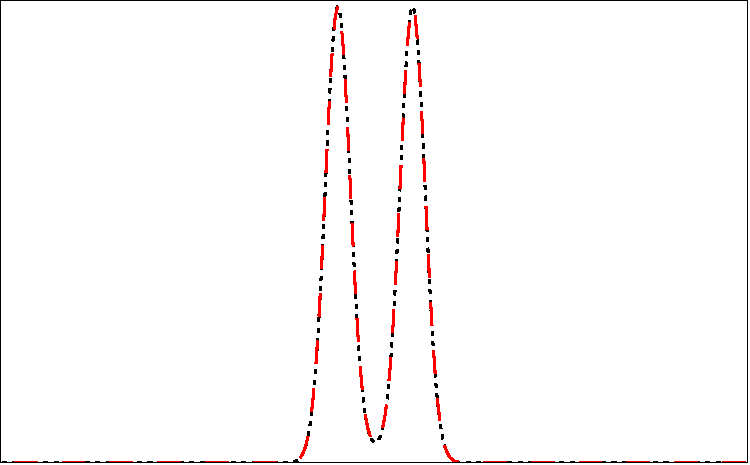
\includegraphics[width=1\textwidth]{Graphics/Probs_ep-10_dd.pdf}
  \caption*{(a)}
\end{minipage}
\begin{minipage}[t]{0.23\textwidth}
\centering
  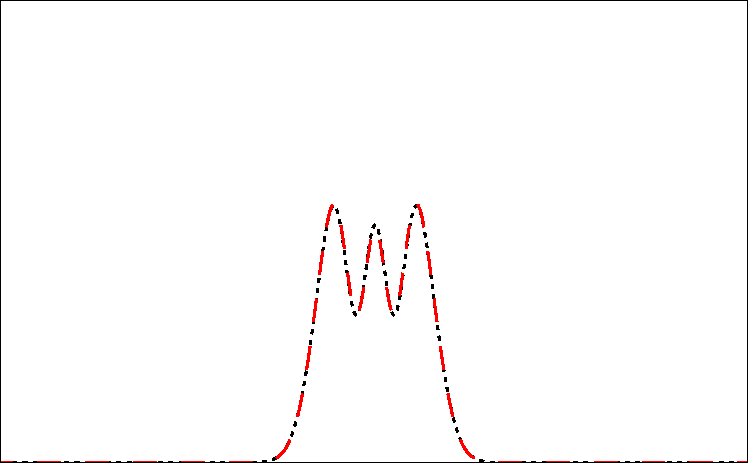
\includegraphics[width=1\textwidth]{Graphics/Probs_ep-98_dd.pdf}
  \caption*{(b)}
\end{minipage}
\begin{minipage}[t]{0.23\textwidth}
\centering
  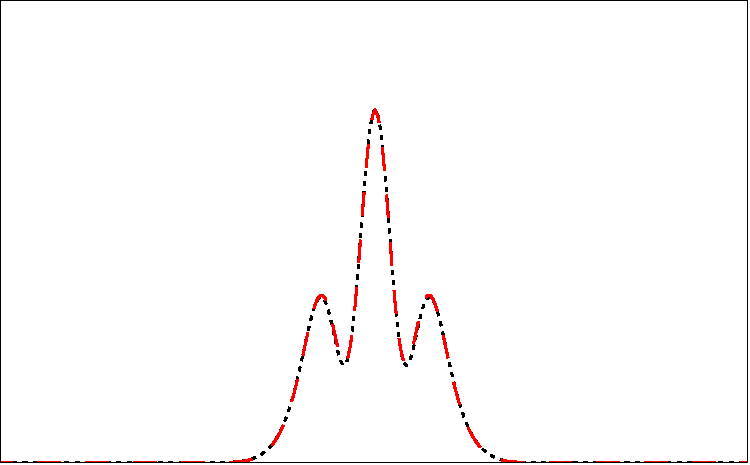
\includegraphics[width=1\textwidth]{Graphics/Probs_ep-95_dd.pdf}
  \caption*{(c)}
\end{minipage}
\begin{minipage}[t]{0.23\textwidth}
\centering
  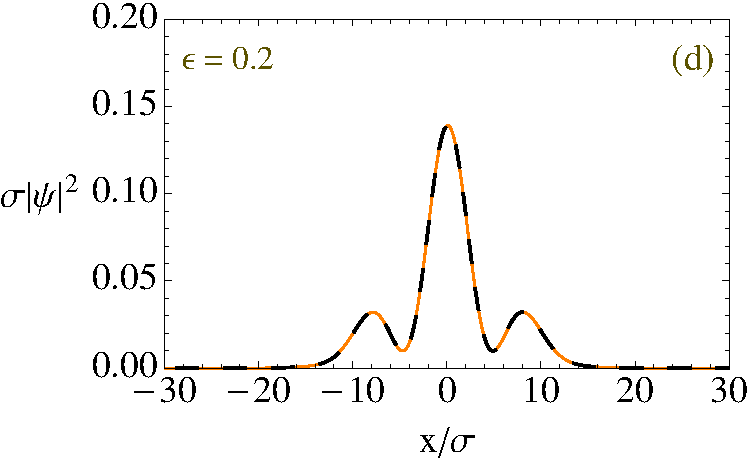
\includegraphics[width=1\textwidth]{Graphics/Probs_ep-8.pdf}
  \caption*{(d)}
\end{minipage}
\begin{minipage}[t]{0.23\textwidth}
\centering
  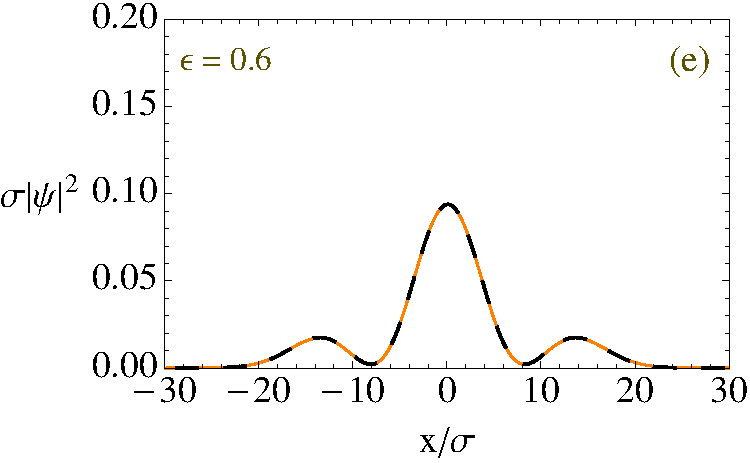
\includegraphics[width=1\textwidth]{Graphics/Probs_ep-4.pdf}
  \caption*{(e)}
\end{minipage}
\begin{minipage}[t]{0.23\textwidth}
\centering
  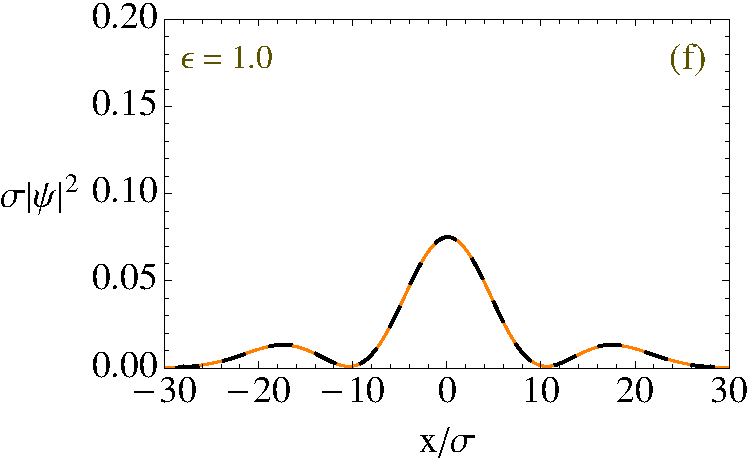
\includegraphics[width=1\textwidth]{Graphics/Probs_ep-0.pdf}
  \caption*{(f)}
\end{minipage}
\caption{Dotted line is the analytic probability using the Schr\"{o}dinger equation with a scaled $\hbar = \tilde{\hbar} \sqrt{\epsilon}$ and the dashed line is the simulated probability using the transition equation.  All plots are evaluated at the same time $t = \tau$. (a) is the fully classical case with $\epsilon = 0$. (b) $\epsilon = 0.02$. (c) $\epsilon = 0.05$. (d) $\epsilon = 0.2$. (e) $\epsilon = 0.6$. (f) is the fully quantum case with $\epsilon = 1$.}
\label{fig:diffract_movie3}
\end{figure}

As can be seen in Fig. (\ref{fig:diffract_movie}) the asymptotic behavior is as expected.  For the completely quantum case, $\epsilon = 1$, the diffraction pattern that forms is identical to the analytic case, Eq. (\ref{eqn:wf_double_t}).  For the completely classical case, $\epsilon = 0$, The diffraction pattern that forms is just that of the initial distribution, Eq. (\ref{eqn:double_init_prob}).

For all values of $0 < \epsilon \leq 1$, given enough time, a far-field diffraction pattern will develop with a visibility of one.  The time for a diffraction pattern to develop increases to infinity as degree of quantumness diminishes, $\epsilon \rightarrow 0$.  The diffraction patterns for the higher values of $\epsilon$ are less developed that for the lower values, but the visibility for all of them is one.  Fig. (\ref{fig:diffract_movie}) shows that the linear Schr\"{o}dinger equation with a scaled $\hbar$ produces completely equivalent results to the numerically solved non-linear transition equation.

\section{Conclusion}

We have demonstrate both analytically and numerically that it is not necessary to get rid of the classicality-enforcing potential to recover quantum behavior.  We have found that by scaling and not necessarily eliminating the classicality-enforcing potential the linear Schr\"{o}dinger equation is recovered, but with a rescaled $\hbar$.


\begin{thebibliography}{4}

\bibitem{bib:bohm}
D. Bohm, \emph{A Suggested Interpretation of the Quantum Theory in Terms of ``Hidden'' Variables}. I, Phys. Rev. 85, 166 (1952).

\bibitem{bib:obm}
X.Oriols and J.Mompart \emph{Overview of Bohmian Mechanics}pages: 15-147; Chapter 1 of the book \emph{Applied Bohmian Mechanics: From Nanoscale Systems to Cosmology} Editorial Pan Stanford Publishing Pte. Ltd (2012).

\bibitem{bib:revisited}
Wolfgang P. Schleich, Daniel M. Greenberger, Donald H. Kobe, and Marlan O. Scully
\emph{Schr�dinger equation revisited}
PNAS 2013 110 (14) 5374-5379; published ahead of print March 18, 2013, doi:10.1073/pnas.1302475110

\bibitem{bib:couder_orbits}
E. Fort, A. Eddi, A. Boudaoud, J. Moukhtar, and Y. Couder, \emph{Path-memory induced quantization of classical orbits}, PNAS 107, 17515 (2010).

%\bibitem{bib:theonlymystery}
%Feynman, Richard P. \emph{Six Easy Pieces} Reading, MA: Addison-Wesley, 1995.

\end{thebibliography}


\end{document}  